The Light Monitoring System (LMS) is a remotely-controlled design upgrade addition to the ECal consisting of a bi-color LED attached to the front of each ECal module. PbWO$_4$ scintillating crystals are relatively radiation tolerant but have a known decrease in light yield after exposure to radiation \cite{Batarin2005543}. This effect is non-uniform in the ECal as a module's geometrical position relative to the beam will result in different levels of radiation. The LMS has the ability to turn individual modules on and off independently which proved useful in checking each channel's functionality and correct cabling. The use of LEDs in a monitoring system for the PbWO$_4$ modules is particularly advantageous because the LEDs can be selected such that the shape and duration of the emitted flash can generate a pulse shape similar to the scintillation effect in the crystal. \cite{battaglieri_ft_clas12}.

Each crystal has a plastic LED holder glued to the front that contains a bi-color LED, model RAPID 56-0352, capable of emitting red and blue light. The use of two different colors allows for the study of different effects in the ECal modules. The blue LED has a wavelength close to the 430~nm emission peak of PbWO$_4$  \cite{battaglieri_ft_clas12} and is used to check for radiation damage in the crystal as this spectrum would be most affected. The red light is not susceptible to the radiation effects in the crystals, but is useful for checking the stability of the  APD gain. 

The LMS consists of four driver boards on each half of the ECal. The four driver boards on each half are connected to one of two main controllers, and each driver can turn on a single LED at a time. The controllers provide communication with the LMS through ethernet and USB interfaces. The controller board for the top half of the ECal also contains the master clock signal that sets the rate at which the LEDs flash. This clock signal is sent to the bottom controller so that the driver boards on the bottom half of the ECal can flash at the same rate, and the clock signal is used to trigger LED events when the DAQ is used. 


During the initial assembly of the ECal, the LEDs were used to study the cross talk between ECal modules. The cross talk between channels was found to be at the level of 2$\pm$1$\%$ and generally occurred in modules of the same row to the immediate left and right of the triggered module. The effect most likely appears due to light leakage out the back face of the crystal where the APD does not cover the entire surface.

The raw waveform response from a red LED signal in a single ECal module is shown in Fig.~\ref{Figure:redSignal}. The raw units are given in mV which are a factor of four times less than the units of FADC.

\begin{figure}[H]
  \centering
      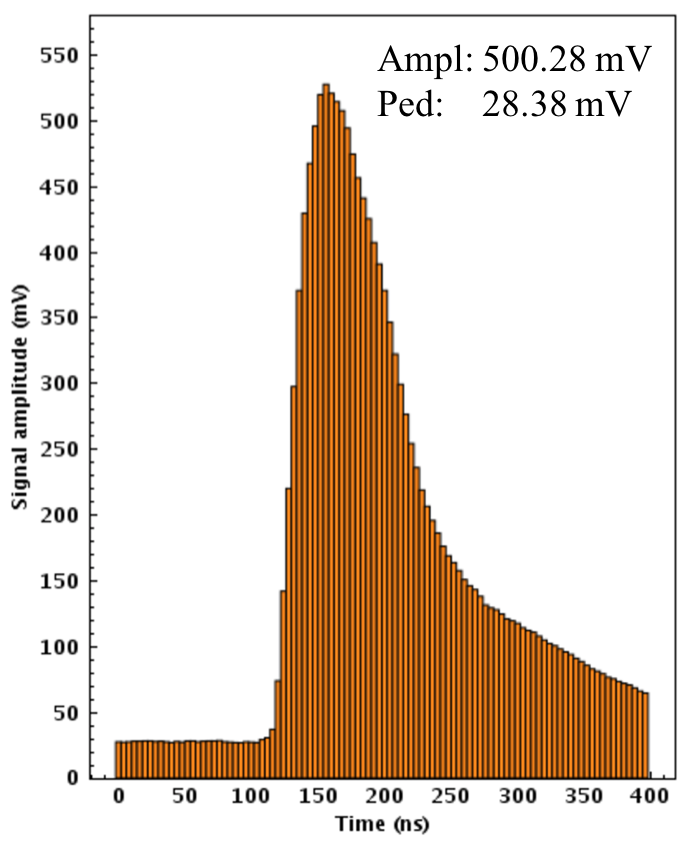
\includegraphics[width=0.5\textwidth]{pics/experiment/ledSignal.png}
  \caption[LED signal in ECal FADC]{A red LED in a single ECal module as readout through the FADC (see section~\ref{pulsefitting})}
  \label{Figure:redSignal}
\end{figure}

Before and after periods of long beam run times, the ECal gains were checked with the LEDs. The LED test ran a sequence of red and blue LEDs so that the characteristic response of each module was measured. The typical results from an LED test are shown in Fig.~\ref{Figure:redCompare}.

\begin{figure}[H]
  \centering
      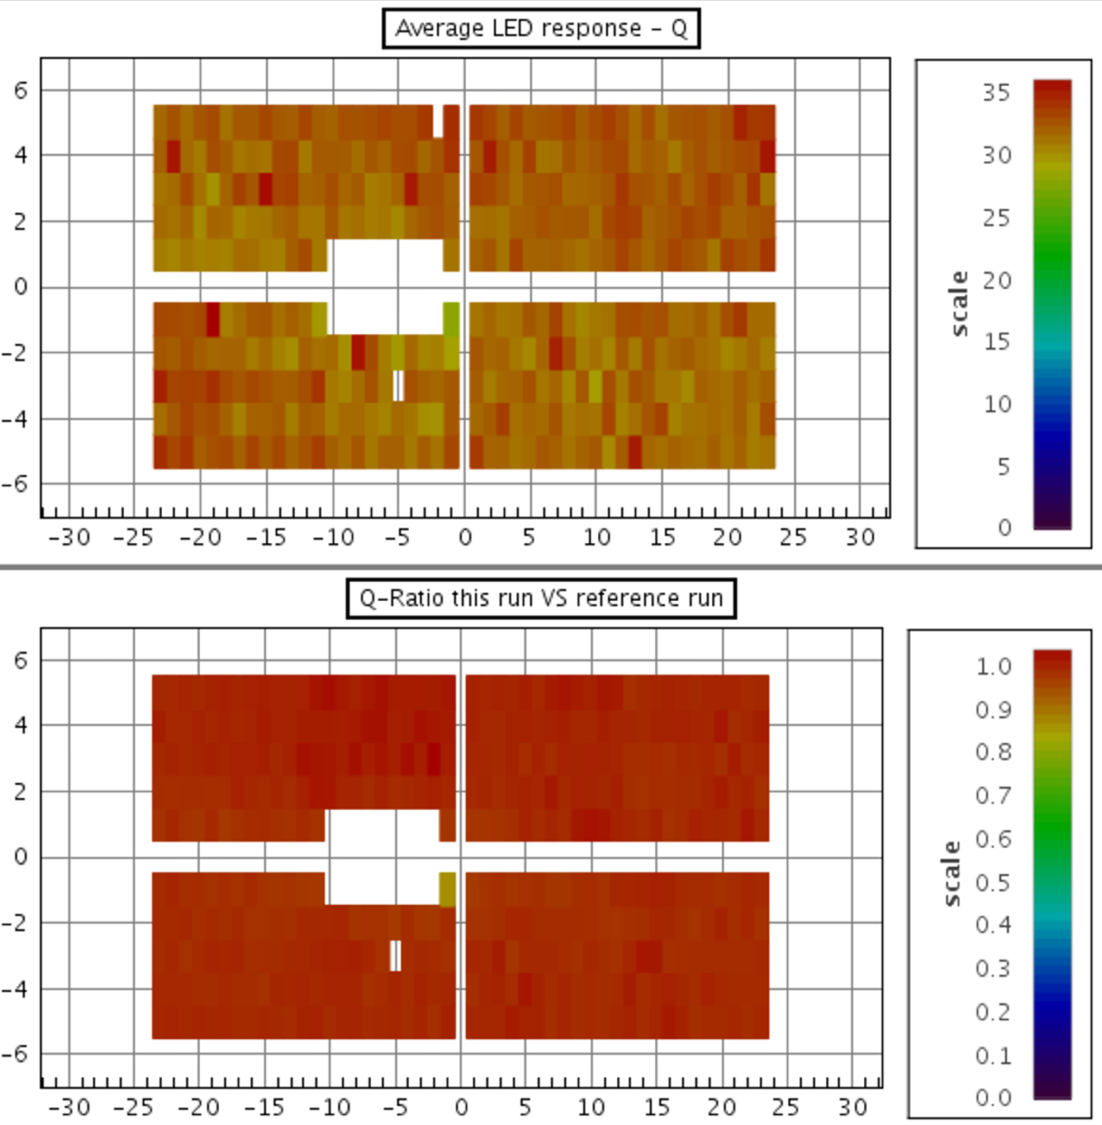
\includegraphics[width=0.5\textwidth]{pics/experiment/ledCompare.png}
  \caption[Results of a single LED run]{The top shows the LED response in each crystal for a specific LED run. The bottom compares each crystal with a its database value as stored from a previous LED run.}
  \label{Figure:redCompare}
\end{figure}

As shown in Fig.~\ref{Figure:redCompare}, the individual ECal module response is given as the pulse-integral in units of GeV. The response values for individual crystals have large units of energy because the LED pulse is significantly longer than an actual scintillation pulse in the crystal. A LED test can show differences in the gain of individual crystals on the order of $1\%$ when compared to previous LED test results. During the Engineering Run, a 5$\%$ change in the gains across all modules occurred over the course of establishing production beam between February and April. This change was seen in LED response studies in addition to the gains obtained with cosmic energy calibration.
